\documentclass[onecolumn]{article}
%\usepackage{url}
%\usepackage{algorithmic}
\usepackage[a4paper]{geometry}
\usepackage{datetime}
\usepackage[margin=2em, font=small,labelfont=it]{caption}
\usepackage{graphicx}
\usepackage{mathpazo} % use palatino
\usepackage[scaled]{helvet} % helvetica
\usepackage{microtype}
\usepackage{amsmath}

\usepackage{subfigure}
\usepackage{subcaption}
% Letterspacing macros
\newcommand{\spacecaps}[1]{\textls[200]{\MakeUppercase{#1}}}
\newcommand{\spacesc}[1]{\textls[50]{\textsc{\MakeLowercase{#1}}}}

\usepackage{graphicx,array}
\newcolumntype{C}[1]{>{\centering\let\newline\\\arraybackslash\hspace{0pt}}m{#1}}
\newcolumntype{L}[1]{>{\raggedright\let\newline\\\arraybackslash\hspace{0pt}}m{#1}}

\title{\spacecaps{DIGIT RECOGNITION REPORT}\\ \normalsize \spacesc{Ceng 3521, Data Mining} }

\author{Can't\_Learn\_Sklearn\\(Ahmet Oral'180709008' - Ceyda Nur Kandemir'170709028' - Onur Yiğit'170709008')\\https://github.com/ahmet-ceng/Digit\_Recognition}
%\date{\today\\\currenttime}
\date{January, 2021}
\begin{document}
\maketitle

\begin{abstract}
In this project we created a program that can identify handwritten digits with more than \%99 accuracy. We used MNIST dataset for training our program. We created 3 .py files; 'saveModel.py', 'evaluateModel.py' and 'predictGUI.py'. In 'saveModel.py' we preprocess the data, normalize images, define and save the model. In 'evaluateModel.py' model can be evaluated. 'predictGUI.py' contains a GUI that user can draw digits with mouse and get predictions.
\end{abstract}

\section{Introduction}
Machines can read the digits written with specific fonts but can't read handwritten digits because each one is different then each other. Goal of this project is to create a Digit Recognition program which can predict output corresponding to handwritten images. We want our program to be not limited by datasets test images so we will implement a GUI for users to draw their digits and make predictions according to those images.



\section{Dataset}

 \begin{tabular}{C{3.8cm}  L{8.8cm}}
        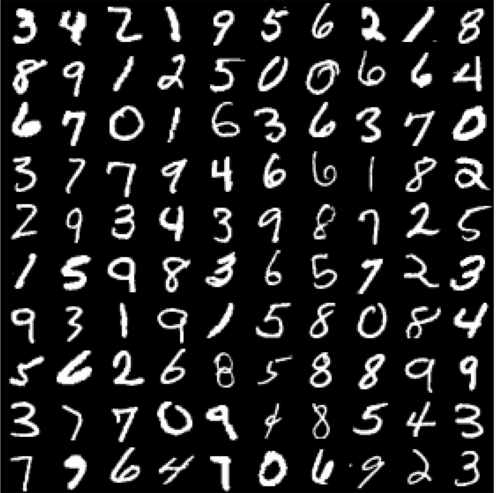
\includegraphics[width=0.9\linewidth]{mnist.png} &  \newline 
        MNIST is a widely used dataset for the hand-written digit classification task. The MNIST stands for the Modified National Institute of Standards and Technology. It consists of 70,000 labelled 28x28 pixel gray scale images of hand-written digits. The dataset is split into 60,000 training images and 10,000 test images. There are 10 classes (one for each of the 10 digits). 
       
    \end{tabular}
\clearpage



\section{Creating and saving the Model (saveModel.py)}
\subsection{Loading and Preprocessing Dataset:}

\par We loaded the data using 'mnist.load\_data()' function. The shape of our training data is (60000, 28, 28). \vspace{5mm} %5mm vertical space
\\To avoid,\\ 
\emph{ValueError: Error when checking input: expected 4 dimensions, but got array with shape (60000, 28, 28)} \vspace{5mm} %5mm vertical space
\par We had to reshape our data to have 4 dimensions. The 2D convolution layer in Keras expects the number of channels (by default as the last dimension). The images are 28x28 and 1 color channel so we reshaped the data arrays to have a single color channel.\vspace{5mm}
\par To able to operate on label data, we used 'One-Hot Code' technique. So all input and output variables are converted to a numerical form.
\begin{figure}[h!]
\centering
    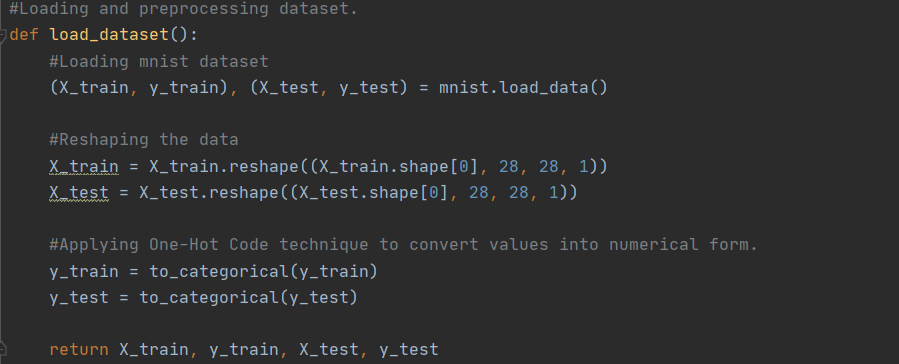
\includegraphics[width=0.6\linewidth]{loading.PNG}
\caption{\label{}
load\_dataset function}
\end{figure}

Pixel values in images have to be scaled to provide the images as input to our CNN model. We needed to normalize inputs from 0–255 to 0–1 as to change the values of numeric columns in the dataset to a common scale, without distorting differences in the ranges of value. To do this, we convert the data type from integers to floats, then divide pixel values by maximum value (which is 255).It helps the model to better learning of features by decreasing computational complexities
\begin{figure}[h!]
\centering
    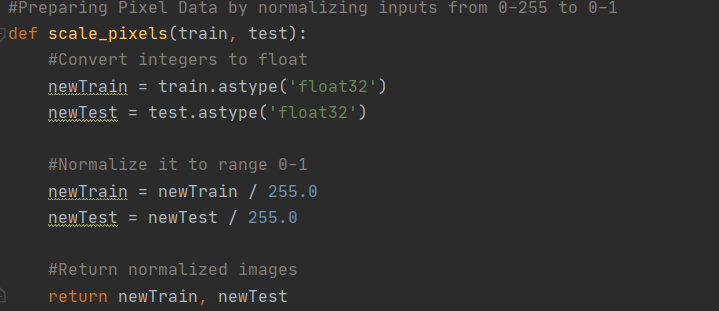
\includegraphics[width=0.6\linewidth]{scaling.PNG}
\caption{\label{}
scale\_pixels function}
\end{figure}

\clearpage
\subsection{Creating Model}

\begin{figure}[h!]
\centering
    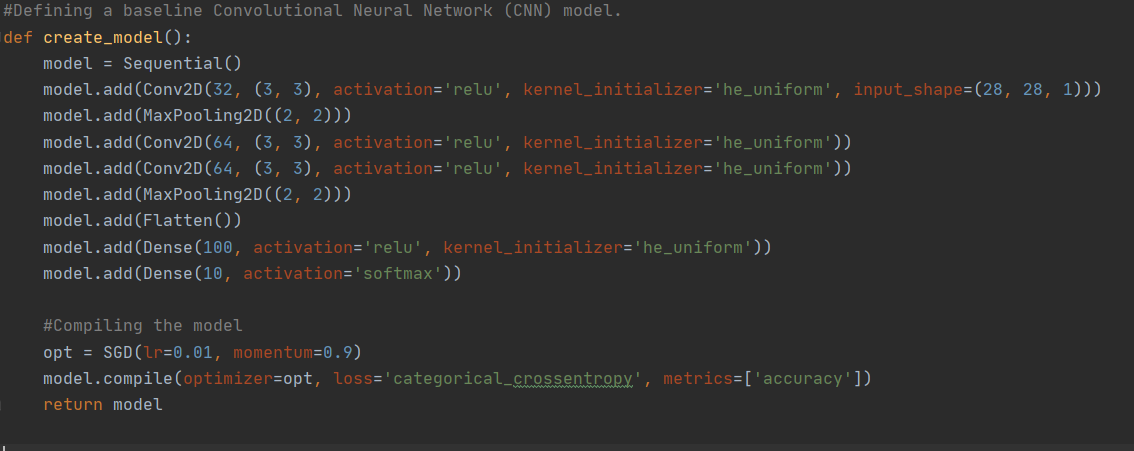
\includegraphics[width=\linewidth]{model.PNG}
\caption{\label{}
scale\_pixels function}
\end{figure}

We defined a baseline convolutional neural network model for the problem.We used Sequential model because it is appropriate for a plain stack of layers where each layer has exactly one input tensor and one output tensor.

There are 2 main aspects in the model, a front end feature extraction  comprised of convolutional and pooling layers, and a classifier backend that going to make a prediction.

For the convolutional front-end, we started with a single convolutional layer with a small filter with '3,3' size, and a '32' number of filters followed by a max pooling layer. To increase model depth we added more convolutional and pooling layers with the same sized filter but we increased the number of filters to '64'.

Our problem is multi-class classification task, and we need an output layer with 10 nodes so that we can predict the probability of distribution of an image that belongs to one of the 10 classes. Because of this, we used softmax activation function. We added a dense layer with 100 nodes to interpret the features between the feature extractor and output layer.

We used 'ReLU' activation function and  'he\_uniform' kernel initializer in all layers because they work the best for this problem.

For optimizer, we used SGD with learning rate of 0.01 and momentum of 0.9. We optimized 'categorical\_crossentropy' loss function because it is suitable for multi-class classification. We monitored the classification accuracy metric because we have the same number of examples in each of the 10 classes.






\clearpage
\subsection{Main Function}
Main is our last function which combines all other functions for preprocessing and creating model. We start by loading the preprocessed dataset using 'load\_dataset()' function. Then we process pixel data using 'scale\_pixels()' function. We load our mode using 'create\_model()' function. After that we fit training dataset to our model and save it as 'model.h5'.

\begin{figure}[h!]
\centering
    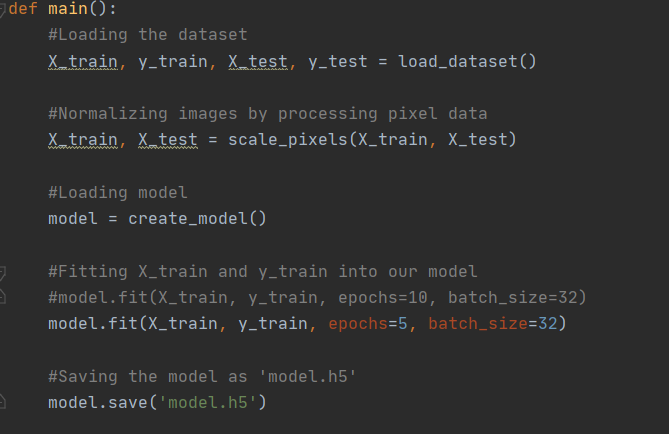
\includegraphics[width=0.6\linewidth]{main.PNG}
\caption{\label{}
main function}
\end{figure}

While fitting the training dataset into our model, we used 5 epochs and 32 batch size. We left the verbose as default so each epoch can be observed. The reason we used 5 epoch is because after around algorithm runs for 4 times accuracy improvement is so little. To save on time we stopped after 5 epochs. The reason we used batch size 32 is because we saw that 32 is balanced value between time and accuracy.

\begin{figure}[h!]
\centering
    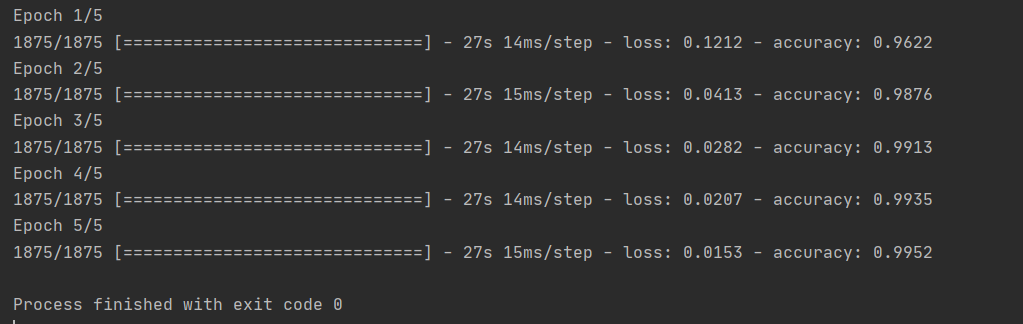
\includegraphics[width=0.7\linewidth]{epoch.PNG}
\caption{\label{}
Fitting the training data in the model}
\end{figure}

It takes around 2 minutes to fit the model and as seen in the picture above, we reached accuracy values more than \%99. After the process we save the model as 'model.h5' so running it one time is enough for the program to work. In our repository we will include our .h5 file if you choose not to wait for this process, you can use our pre fitted model.
\clearpage



\section{Evaluating the Model (evaluateModel.py)}
We load and preprocess the data as we did in 'saveModel.py'. Inside the main function, we load the model we crated before. We used model.evaluate() function to evaluate the model on the test dataset. Then we printed the accuracy and loss.
\vspace{5mm}
\par After running evaluateModel.py the you can see the accuracy and loss of the model.
\begin{figure}[h!]
\centering
    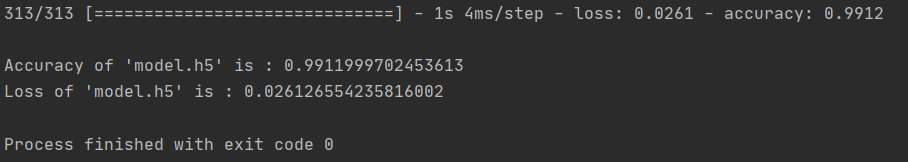
\includegraphics[width=0.8\linewidth]{evaluate.PNG}
\caption{\label{}
Loss and Accuracy of the model}
\end{figure}

\section{Creating GUI and Making Predictions (predictGUI.py)}

We used tkinter to create our gui because we were already familier with it and it reuqires all of our needs. \par We created 4 functions called 'load\_prepare\_predict()', 'painting(event)', 'btnPredict()' and 'btnClear()'. 

\subsection{load\_prepare\_predict() Function:}
\begin{figure}[h!]
\centering
    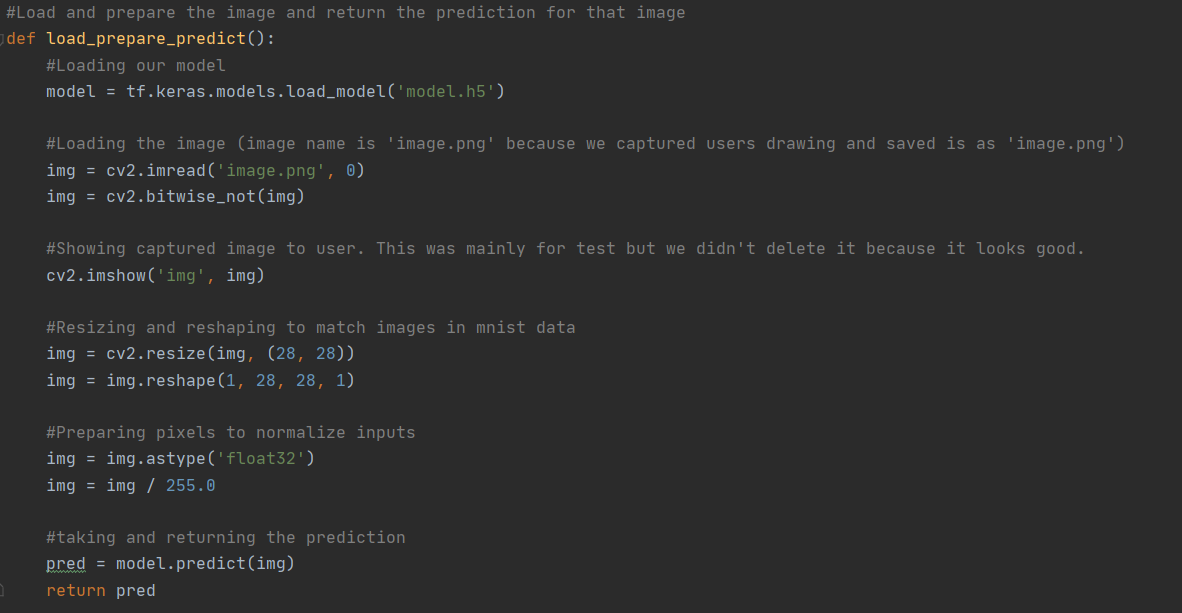
\includegraphics[width=0.8\linewidth]{func1.PNG}
\caption{\label{}
load\_prepare\_predict() Function}
\end{figure}

In this function, we load our model and image. Image name is 'image.png' because when we call this function we will be already saved our image as 'image.png'. We process the image by resizing and reshaping. Then as we did in our saveModel.py file, we prepare the pixels by converting it to float and normalizing it to range 0-1. Then we use '.predict()' function to get prediction of the image using our model and return it.
\clearpage

\subsection{btnPredict() function:}
\begin{figure}[h!]
\centering
    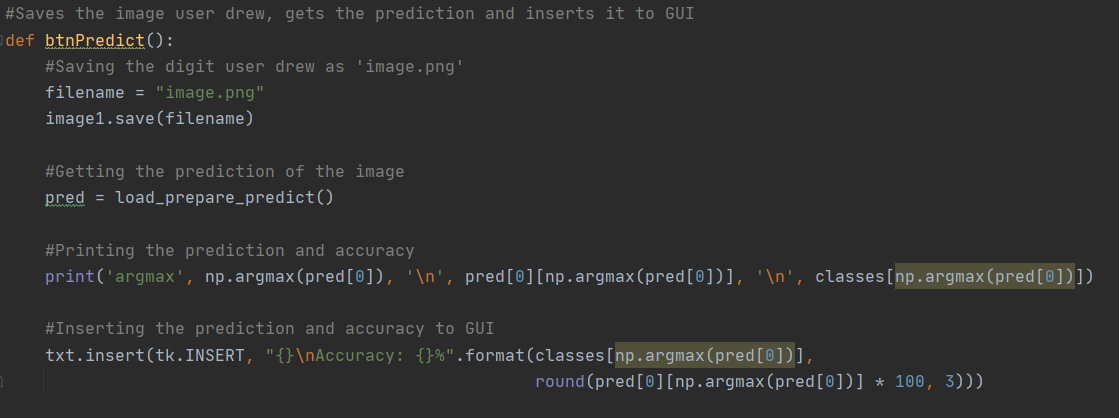
\includegraphics[width=0.8\linewidth]{predictbtn.PNG}
\caption{\label{}
btnPredict() function}
\end{figure}

This function is called when user clicks the 'Predict' button on GUI. We save the digit user drew as 'image.png' and get the prediction by calling 'load\_prepare\_predict()' function. Then we print(in console) and display(in GUI) accuracy and prediction of the image.


\subsection{btnClear() function:}
\begin{figure}[h!]
\centering
    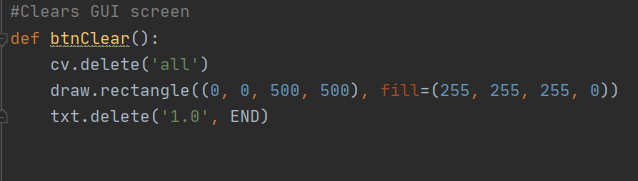
\includegraphics[width=0.6\linewidth]{clear.PNG}
\caption{\label{}
btnClear() function}
\end{figure}

This function is called when user clicks 'Clear' button. It clears the canvas where user drew, and text area where predictions displayed.

\subsection{painting() function:}
\begin{figure}[h!]
\centering
    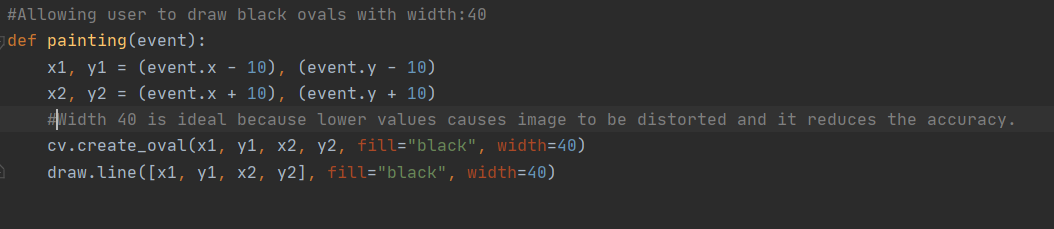
\includegraphics[width=0.6\linewidth]{painting.PNG}
\caption{\label{}
painting() function}
\end{figure}

This function is called when user uses mouse1. It creates black ovals with 40 width to where user points the mouse. Width 40 look a little big when drawing. But lower width values causes our image to be distorted and reduces the accuracy.


\clearpage
\subsection{GUI Design}
\begin{figure}[h!]
\centering
    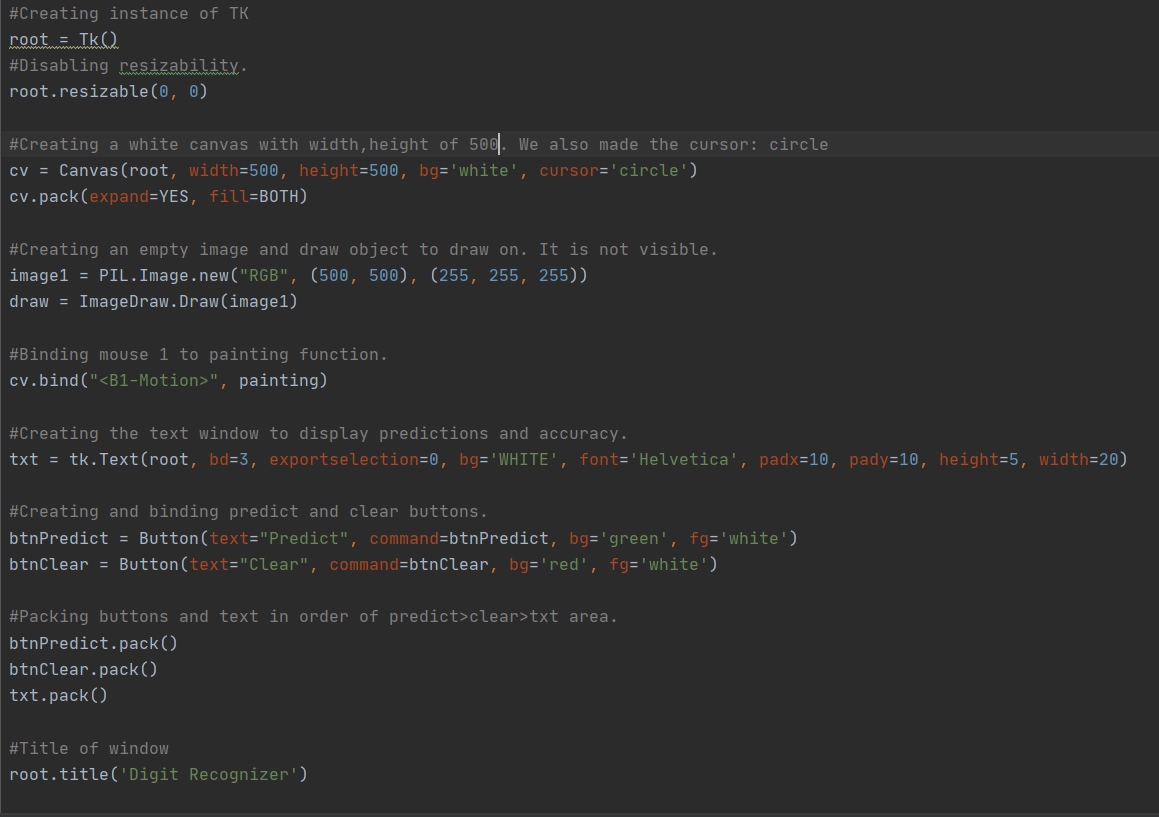
\includegraphics[width=0.9\linewidth]{gui.PNG}
\caption{\label{}
Creating GUI}
\end{figure}

We disabled option to resizing window because if user resizes the window image gets distorted and it causes problems.

We created a white canvas with 500 width and heigt (it looks best with 500) and changed the cursor to circle so it looks different in GUI.

To save the image user drew, we created an empty image and draw object to draw on. It is not visible to the user (User see it as they are drawing on GUI) and has the same width and height as the canvas we created.

We bind mouse1 to painting function so user can drew. Then we created a text small text area to display predictions and accuracy, 

We created 2 buttons called predict and clear. Predict button runs the 'btnPredict()' function which save the image user drew and calls 'load\_prepare\_predict()' function to get predictions. Then it displays the results in GUI. Clear button calls the 'btnClear' function which clears the canvas and text area. We also colored the buttons so they look nice.

Finally we packed buttons and text are and set the title of our GUI.




\vspace{45mm}

\subsection{GUI and Testing}

\begin{figure}[h!]
  \centering
  \begin{minipage}[b]{0.3\textwidth}
    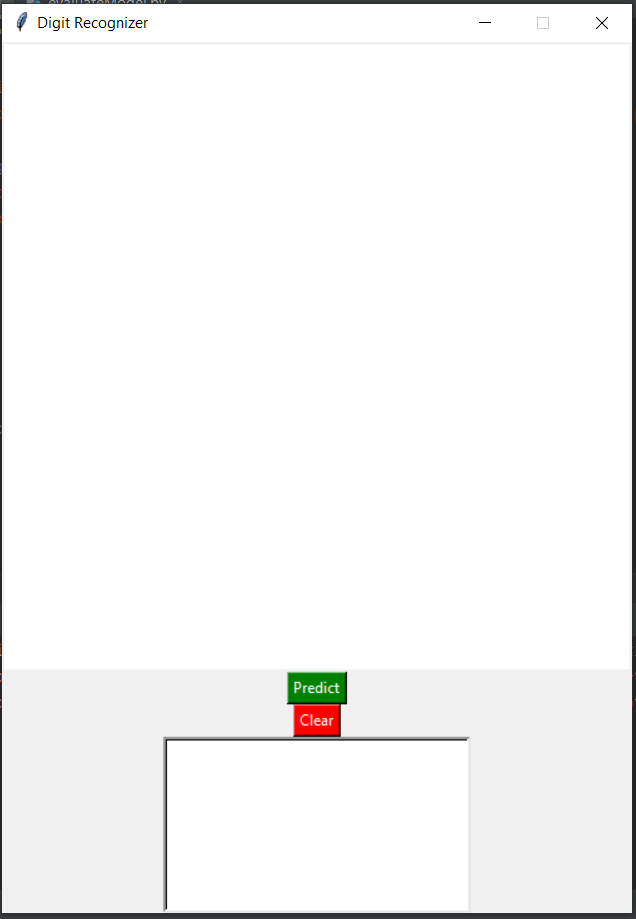
\includegraphics[width=\textwidth]{gui2.PNG}
    \caption{Empty GUI}
  \end{minipage}
  \hfill
  \begin{minipage}[b]{0.6\textwidth}
    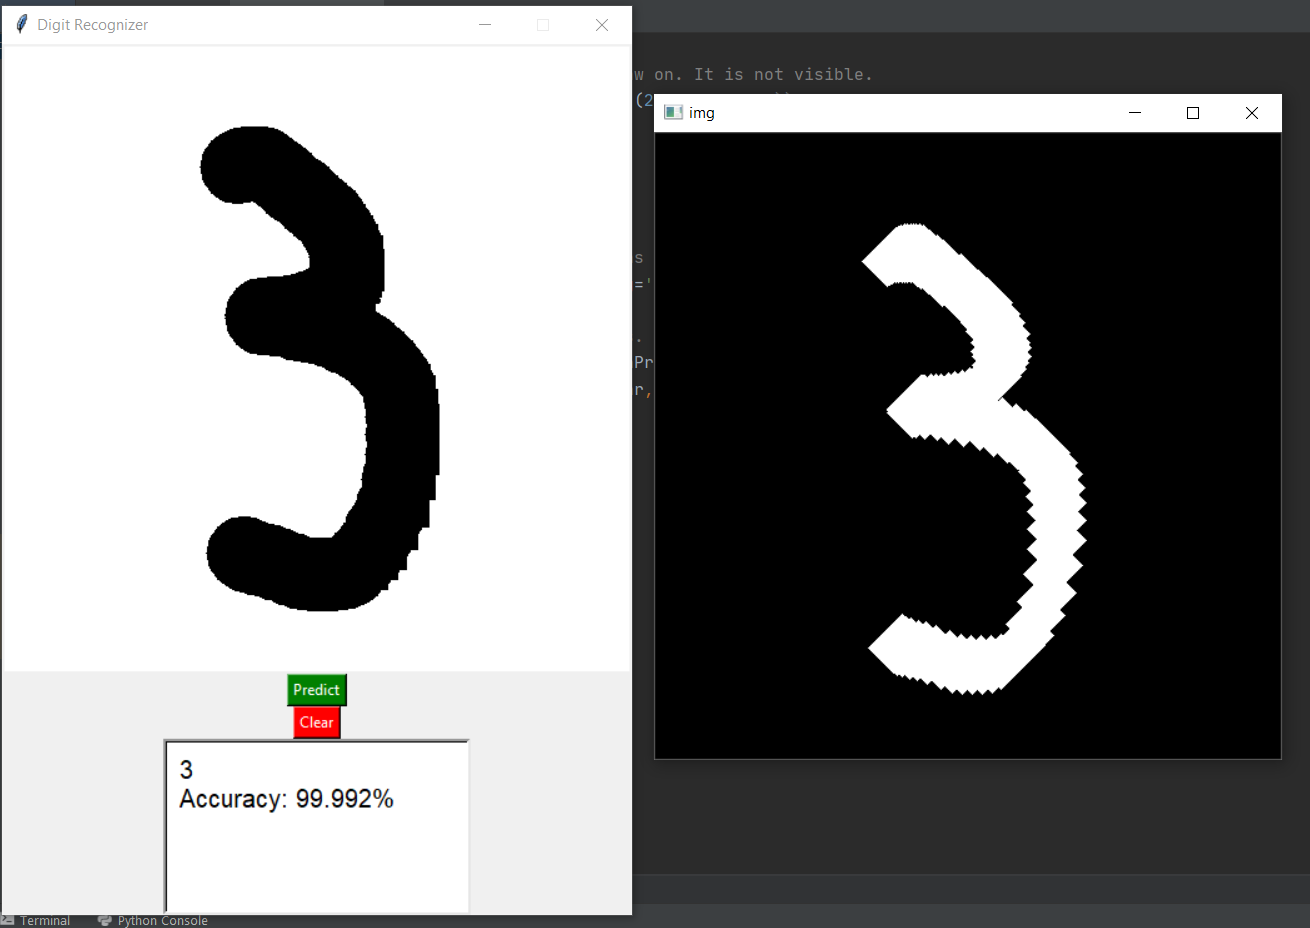
\includegraphics[width=\textwidth]{test.PNG}
    \caption{GUI Test}
  \end{minipage}
\end{figure}

Our GUI looks like in the figure11 when empty.It has 2 buttons which are predict and clear. Predict button displays the prediction and accuracy, clear button clears the canvas and text area. 

On figure12 there is an example of drawing and getting prediction. As you can see we drew 3 with our mouse and after clicking predict button, in the text area below you can see it predicts 3 with \%99 accuracy. The black and white image on the left is the image captured by the machine. It is processed and used to get predictions.
\vspace{5mm}


 \begin{tabular}{C{3.8cm}  L{8.8cm}}
        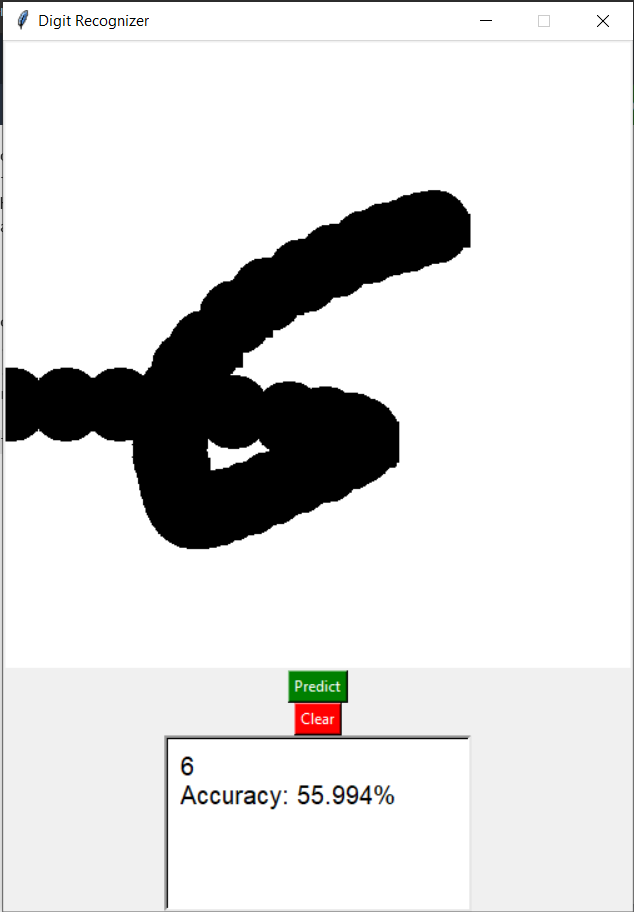
\includegraphics[width=0.9\linewidth]{test1.PNG} &  \newline 
        We did a lots of testing. If written clearly, program correctly reads the digit with more than \%99 accuracy. If handwritten is really bad, but still readable to humans, program still can accurately read most of the times(for ex. figure on left). If you randomly paint something it gets confused and fails with prediction and accuracy.
       
       
    \end{tabular}

\clearpage

\section{Conclusion}

In this assignment, using MNIST dataset, we trained a program to predict handwritten digits and it can predict test dataset with more than \%99 accuracy. We also created a GUI for predicting real handwritten digits, not just the datasets test images. Images we created with mouse in our GUI also reached around \%99 accuracy (if it was drawn good). Even if we draw very bad, we managed to get very good predictions.

We learned to process data to make it usable in CNN, we learned to construct a Convolutional Neural Network model, we learned a method called One-Hot Code to make labels operatable, we learned normalisation to reduce the scale of the input values, we learned to reshape the array of pixels so we can feed it into CNN.

In this assignment we tried to approach problems in different ways and we always tried to improve our code.We used our own knowledge and when it is not enough to solve a problem we learned new methods to solve it. We tried to write our code as clean as possible and we added comments to describe each piece of code.

All in all this assignment contributed lots of new skills to us and we enjoyed doing it.
\end{document}
